\documentclass[japanese,draft]{jssst_ppl} %% $BF|K\8l(B (default)
% \documentclass[english]{jssst_ppl} %% English
% \documentclass[japanese,draft]{jssst_ppl} %% You can use the draft option

\title{algebraic effect handlers $B$r4^$`%W%m%0%i%`$N%9%F%C%W<B9T(B}
\author{$B8E@n(B $B$D$-$N(B, $B@u0f(B $B7r0l(B}
\inst{
  $B$*Cc$N?e=w;RBg3X(B\\
\texttt{furukawa.tsukino@is.ocha.ac.jp, asai@is.ocha.ac.jp}
}
\begin{document}
\maketitle
\begin{abstract}
$B%9%F%C%Q$O%W%m%0%i%`$N<B9T2aDx$r8+$;$k%D!<%k$G$"$k!#$3$l$^$GMM!9$J8@8l$KBP$9$k%9%F%C%Q$,:n$i$l$F$-$?$,!"(Bshift/reset $B$d(B algebraic effect handlers $B$H$$$C$?7QB3$rL@<(E*$K07$&8@8l5!G=$r%5%]!<%H$9$k%9%F%C%Q$O:n$i$l$F$$$J$$!#7QB3$r07$&%W%m%0%i%`$N5sF0$rM}2r$9$k$N$O:$Fq$J$N$G!"$=$&$$$C$?8@8l$KBP1~$7$?%9%F%C%Q$r:n$k$3$H$,K\8&5f$NL\E*$G$"$k!#(B
$B%9%F%C%Q$O4JLs$N$?$S$K$=$N;~E@$G$N%W%m%0%i%`A4BN$r=PNO$9$k%$%s%?%W%j%?$J$N$G!"<B9T$7$F$$$kItJ,<0$N%3%s%F%-%9%H$N>pJs$,>o$KI,MW$K$J$k!#7QB3$r07$&$h$&$JJ#;($J5!G=$r;}$D8@8l$rBP>]$K$7$?%9%F%C%Q$G$O!"%3%s%F%-%9%H$,$I$N$h$&$J9=B$$r$7$F$$$k$+$,<+L@$G$J$$!#$=$3$G!"DL>o$N%$%s%?%W%j%?4X?t$r%W%m%0%i%`JQ49$9$k$3$H$G5!3#E*$K%3%s%F%-%9%H$N>pJs$rJ];}$5$;!"%9%F%C%Q$r<BAu$9$kJ}K!$r<($9!#(B
$B<B:]$K7?L5$7&K7W;;$H(B algebraic effect handlers $B$+$i@.$k8@8l$K$D$$$F<BAuJ}K!$r<($7!"$=$l$r$b$H$K$7$F<BAu$7$?(B Multicore OCaml $B$rBP>]$H$7$?%9%F%C%Q$r>R2p$9$k!#(B
\end{abstract}

\section{はじめに}

書いたプログラムが思った通りの挙動をしない時、プログラマはデバッグをする必要がある。

単純なデバッグはプログラムを実行した際の出力から推測したりソースコードを眺めることで行われるが、そのようなデバッグは「ソースコードのどの部分が間違っているか」を示すものが無く、多くの時間や労力を要することがある。特にプログラミングにまだ慣れていない初学者にとっては、デバッグの経験や言語に対する理解が乏しい為、より困難な作業になると考えられる。

そこで色々な言語にデバッガが用意されているが、デバッガを利用するには、デバッガのコマンドの文字列や意味を覚えたり、ブレイクポイントを設定する箇所を考えたりといった、初学者にとってやはり困難な操作が必要になる。また、一般的なデバッガで表示されるのは「ソースコード中の実行中の行」であり、どこで今の関数を呼び出されたのか、この後どんな計算があるのかなどといったプログラム全体の流れが分かりにくい。

\begin{figure}
  \begin{center}
    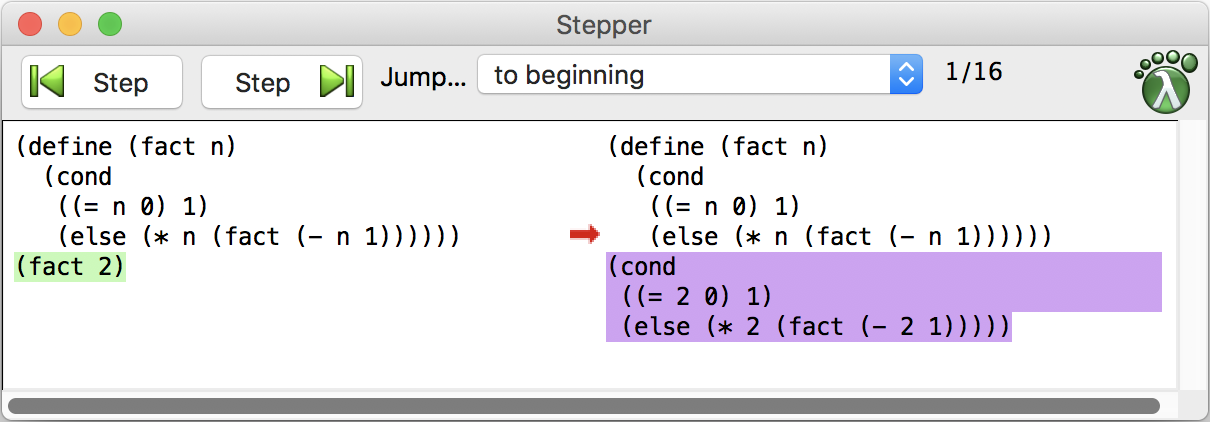
\includegraphics[width=13cm]{racket1.png}
  \end{center}
  \caption{DrRacket のステッパ}
  \label{figure:racket1}
\end{figure}

\begin{figure}
  \begin{center}
    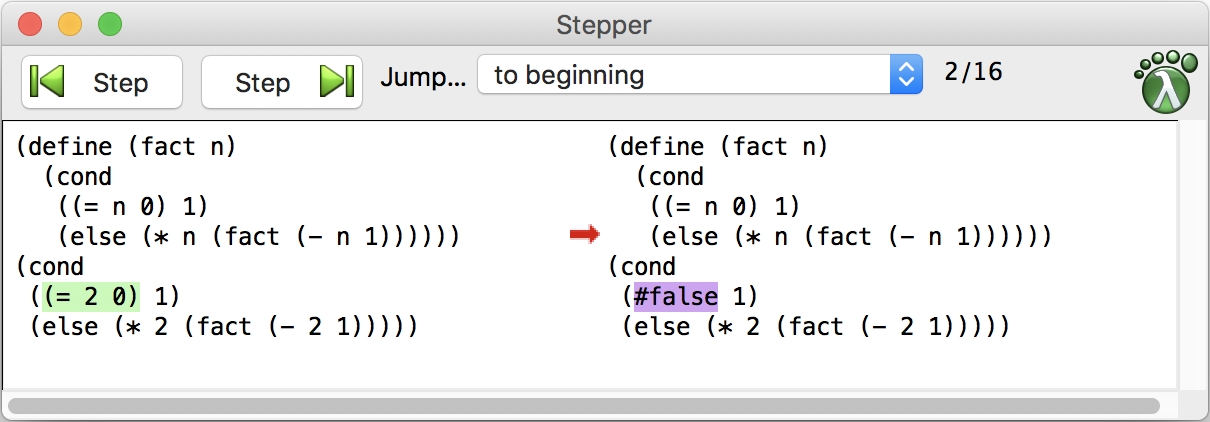
\includegraphics[width=13cm]{racket2.png}
  \end{center}
  \caption{DrRacket のステッパを進めた様子}
  \label{figure:racket2}
\end{figure}

我々は、プログラミング初心者がデバッグをするのに最適な方法は、ステッパを使うことだと考える。ステッパは Racket 言語の統合開発環境 DrRacket において提供されているツール\cite{clements01}である。ユーザがエディタにプログラムを書いてステッパ起動ボタンを押すと、図\ref{figure:racket1}のようなウインドウが表示される。図\ref{figure:racket1}は、再帰関数を用いて2の階乗を計算するプログラムを入力してステッパを起動したときの様子である。ウインドウには左右にそれぞれプログラムが表示されている。左はユーザが入力したプログラムと同じものであり、このプログラムで最初に簡約される式 \texttt{(fact 2)} が緑色にハイライトされている。右側のプログラムでは、ハイライトされた部分以外は左側と同じプログラムが表示されており、左側では緑色だった式 \texttt{(fact 2)} がその簡約結果に置き換えられ、紫色でハイライトされている。

Step ボタンのうち右の実行を進めるボタンを押すと図\ref{figure:racket2}のような表示に切り替わる。最初(図\ref{figure:racket1})は右側にあったプログラムと同じプログラムが左に表示され、次に簡約される部分式 \texttt{(= 2 0)} が緑色にハイライトされており、右側には同様にその部分が簡約されて紫色になったプログラムが表示されている。当初 \texttt{(fact 2)} だった式がその値である \texttt{2} になるステップまで、ボタンを押すと次々に簡約が行われてプログラムが変形していく様子を視覚的に見ることができる。

このように、プログラムを実行したときに、実行結果の値だけでなく、実行中にプログラムが代数的にどのように書き換えられていくかを見せるツールがステッパである。ステッパの操作は基本的に「前のステップへ」「次のステップへ」のボタンを押すのみであり、プログラミングや CUI での操作に慣れていない初心者でも使いやすい。

しかし、DrRacket のステッパが受け付けるのは Racket 言語のうちの一部の構文で構成された教育用の言語であり、例外処理などがサポートされていない。初心者にとって理解しにくい例外処理をステップ実行できるようにするため、著者らは関数型言語 OCaml の、try-with を含む基礎的な構文に対応したステッパを実装し評価した\cite{FCA19}。

本研究の目的は、継続を明示的に扱うことができる言語機能を含む言語に対応したステッパを作ることである。
shift/reset \ref{?} や algebraic effects \ref{?} といった継続を扱う言語機能を含むプログラムの挙動は複雑で理解が困難だが、継続を値として扱うことができる言語機能に対応したステッパはまだ作られていない。

ステッパは簡約により書き換わっていくプログラム全体を出力するインタプリタなので、ステッパを実装する際には、部分式を再帰的に実行している時にそのコンテキストの情報を得ることが必要になる。以前の研究\cite{FCA19}では評価順序をもとにコンテキストの構造を考えてコンテキストを表すデータ型を定義していたが、本研究ではインタプリタ関数に CPS 変換 \cite{?} および非関数化 \cite{?} という変換を施すことでコンテキストの情報を引数に持つインタプリタ関数を導出し、それを用いてプログラム全体を再構成して出力する方法を提案する。


%\section{ステッパの実装におけるコンテキスト}
\section{ステッパの実装方法とコンテキスト}
\label{section:context}

%ステッパは簡約のたびに簡約前後のプログラムを出力するインタプリタである。例えばプログラム \texttt{((fun a -> a) ((fun b -> b) (fun c -> c)))} を入力した場合、以下のように出力したい。

%\begin{quote}
%\begin{verbatim}
%((fun a -> a) ((fun b -> b) (fun c -> c)))
%((fun a -> a) (fun c -> c))
%
%((fun a -> a) (fun c -> c))
%(fun c -> c)
%\end{verbatim}
%\end{quote}

ステッパは small-step による実行と同じなので、small-step のインタプリ
タを書けば実装できる。実際、Whitington \& Ridge \cite{EPTCS294.3} は small-step のインタプリ
タを書くことで OCaml に対するステッパを実装している。
しかし、small-step のインタプリタをメンテナンスするのは簡単ではない。
また、ステップ実行中に関数呼び出し単位でスキップする機能をつけようと思
うとインタプリタは big-step で書かれていた方が都合が良い。そこで、我々
の過去の研究 \cite{FCA19} では、big-step のインタプリタを元にして
ステッパを作成している。ここでも、そのアプローチをとる。

図 \ref{figure:lambda} に OCaml による型無し$\lambda$計算の定義と代入
ベースの big-step インタプリタの実装を示す。
関数 \texttt{subst :\ e -> (string * v) list -> e} は代入関数であり、
\texttt{subst e [(x, v)]} は式 \texttt{e} の中の
全ての変数 \texttt{x} を値 \texttt{v} に置換した式を返す。

%ステッパはインタプリタにステップ出力機能が加わったものなので、通常のインタプリタ関数に書き加えることで実装できる。図 \ref{figure:lambda} に OCaml による型無し$\lambda$計算の定義とインタプリタの実装を示す。関数 \texttt{subst : e -> (string * v) list -> e} は代入関数であり、\texttt{subst e [(x, v)]} は式 \texttt{e} の中の全ての変数 \texttt{x} を値 \texttt{v} に置換した式を返す。

%ステッパは small-step での実行過程を見せるものであるが、small-step でなく big-step のインタプリタを基にして作ることで、関数適用や配列に対する処理やループ等のひとまとまりの実行の開始と終了を検知して「その部分の最後のステップまで飛ばす」等の機能を作ることが容易になる\ref{FCA19}ため、big-step のインタプリタを利用している。

\begin{figure}
\begin{verbatim}
(* 値 *)
type v = Var of string      (* x *)
       | Fun of string * e  (* fun x -> e *)

(* 式 *)
type e = Val of v      (* 値 *)
       | App of e * e  (* e e *)

(* インタプリタ *)
let rec eval (exp : e) : v = match exp with
  | Val (v) -> v  (* 値ならそのまま返す *)
  | App (e1, e2) ->
    (let v2 = eval e2 in  (* 引数部分を実行 *)
     let v1 = eval e1 in  (* 関数部分を実行 *)
     let reduct = match v1 with
       | Fun (x, e) -> subst e [(x, v2)]  (* 代入 e[v2/x] *)
       | _ -> failwith "type error" in  (* 関数部分が関数でなければ型エラー *)
     eval reduct)  (* 代入後の式を実行 *)
\end{verbatim}
\caption{型無し$\lambda$計算とそのインタプリタ}
\label{figure:lambda}
\end{figure}

このインタプリタをステッパにするには、簡約をする際に簡約前後のプログラ
ムを出力する機能を追加すればよい。
しかしステッパが出力したいのは実行中の部分式ではなく式全体であり、コン
テキストを含めた式全体を出力するためには、実行中の式の構文木の他にコン
テキストの情報が必要である。

%このインタプリタをステッパにするには、簡約をする際に簡約前後のプログラムを出力する機能を追加すればよい。
%関数 \texttt{eval} は実行する式の部分式を再帰的に実行する。すると、再帰呼び出しされた \texttt{eval} の中では、引数に実行中の部分式の情報しか与えられていない。
%しかしステッパが出力したいのは実行中の部分式ではなく式全体であり、コンテキストを含めた式全体を出力するためには、実行中の式の構文木の他にコンテキストの情報が必要である。

コンテキストの情報を得るために、Clements ら\cite{clements01} は Racket
の continuation mark を使用してコンテキストフレームの情報を記録するこ
とでステッパを実装した。本研究ではそのような特殊な機能は使わずに、
インタプリタ関数に明示的にコンテキスト情報のための引数を追加する。
図\ref{figure:lambda}のインタプリタに
その変更を施すと、図\ref{figure:lambda_stepper}のようになる。ここで、
関数 \texttt{memo :\ e -> e -> c -> unit} は、簡約前の式、簡約後の式、
コンテキスト情報の3つを引数にとり、コンテキスト情報を利用して簡約前後
の式全体をそれぞれ出力するものである。

%コンテキストの情報を得るために、Clements ら\cite{clements01} は Racket の continuation mark を使用してコンテキストフレームの情報を記録したが、本研究ではインタプリタ関数に明示的にコンテキスト情報のための引数を追加する。筆者らは以前\cite{FCA19}、実際にインタプリタに引数を追加することによってステッパを実装した。図\ref{figure:lambda}のインタプリタにその変更を施すと、図\ref{figure:lambda_stepper}のようになる。ここでは関数 \texttt{memo :\ e -> e -> c -> unit} は、簡約前の式、簡約後の式、コンテキスト情報の3つの引数をとり、コンテキスト情報を利用して簡約前後の式にそれぞれコンテキストを付加することで簡約前後の式全体を得て出力する。

\begin{figure}
\begin{verbatim}
(* コンテキスト *)
type c = CId             (* [.] *)
       | CApp2 of e * c  (* [e [.]] *)
       | CApp1 of v * c  (* [[.] v] *)

(* 出力しながら再帰的に実行 *)
let rec eval (exp : e) (c : c) : v = match exp with
  | Val (v) -> v
  | App (e1, e2) ->
    (let v2 = eval e2 (CApp2 (e1, c)) in  (* コンテキストを1層深くする *)
     let v1 = eval e1 (CApp1 (v2, c)) in  (* コンテキストを1層深くする *)
     let redex = App (Val v1, Val v2) in
     let reduct = match v1 with
       | Fun (x, e) -> subst e [(x, v2)]
       | _ -> failwith "type error" in
     memo redex reduct c;                 (* コンテキストを利用して式全体を出力 *)
     eval reduct c)

(* 実行を始める *)
let stepper (exp : e) = eval exp CId
\end{verbatim}
\caption{型無し$\lambda$計算に対するステッパ}
\label{figure:lambda_stepper}
\end{figure}

図\ref{figure:lambda_stepper}のように、コンテキストを表すデータ型を定
義して再帰呼び出し時の構造に合わせて引数として渡すようにすれば、式全体
を再構成して出力することが可能になる。ここで、コンテキストを表すデータ
型は、評価文脈そのものになっていることに気がつく。評価文脈のデータ型は、
big-step のインタプリタを CPS 変換し、非関数化すると機械的に得られるこ
とが知られている。これは、我々が手動で定義したコンテキストのデータは、
機械的に導出できることを示唆している。

$\lambda$計算に対するステッパであれば、手動でコンテキストの型を定義す
るのは簡単だが、言語が複雑になってくると必ずしもこれは自明ではない。実
際、以前の研究 \cite{FCA19} で try-with 構文を含む言語のステッパを実装
したときには、コンテキストを try-with 構文で区切る必要があったため、
コンテキストの構造が一次元的でなく、リストのリストになった。
algebraic effects などが入った場合、どのようなコンテキストを使えば良い
のかはまた別途、考慮する必要がある。このような場合、機械的にコンテキス
トの定義を導出できることにはメリットがある。
次節以降ではそのような方針で algebraic effects に対するステッパを導出
する。

%図\ref{figure:lambda_stepper}のように、コンテキストを表すデータ型を定義して再帰呼び出し時の構造に合わせて引数として渡すようにすれば、式全体を再構成して出力することが可能になる。以前の研究 \cite{FCA19} ではこの方法を用いて try-with 構文を含む言語のステッパを実装することに成功した。
%しかし、try-with のような制御構文を含む言語では、コンテキストを区切ってある区間のコンテキストを一度に捨てるなどの操作が必要になるため、コンテキストの構造が一次元的でなくなり、複雑なデータ構造の定義が必要になる可能性がある \cite{FCA19} 。

%ところが、図\ref{figure:lambda_stepper}の\texttt{c}型の定義を見ると、各コンストラクタはインタプリタ関数の「どの再帰呼び出しか」に対応している。コンテキストの型は評価順序によって定まるものであり、評価順序はインタプリタ関数で定義されているので、コンテキストを表すデータ型の定義はインタプリタ関数から導出できるものであると考えられる。次節以降ではその導出方法の1つを提案する。


\section{継続渡し形式のインタプリタ}
\label{section:definition}

この節では、ステッパの対象言語とそのインタプリタを定義する。

\subsection{algebraic effects}
\label{subsection:algebraic effects}



\subsection{対象言語の構文}
\label{subsection:syntax}

対象言語の OCaml による定義を図 \ref{figure:syntax} に示す。型 \texttt{v} に含まれる \texttt{Cont} は継続を表すコンストラクタであり、入力プログラムに含まれることはないが、ステップ実行の過程で現れる。\texttt{Cont} の第一引数の文字列は関数のように表示する際の仮引数名であり表示の為に用いる。

\begin{figure}
\begin{verbatim}
(* 値 *)
type v = Var of string              (* x *)
       | Fun of string * e          (* fun x -> e *)
       | Cont of string * (k -> k)  (* 継続 fun x => ... *)
(* ハンドラ *)
and h = {
  return : string * e;                       (* handler {return x -> e,      *)
  ops : (string * string * string * e) list  (*          op(x; k) -> e, ...} *)
}
(* 式 *)
and e = Val of v          (* v *)
      | App of e * e      (* e e *)
      | Op of string * e  (* op e *)
      | With of h * e     (* with h handle e *)
(* 継続 *)
and k = v -> a
(* 実行結果 *)
and a = Return of v
      | OpCall of string * v * k

\end{verbatim}
\caption{対象言語の定義}
\label{figure:syntax}
\end{figure}


\section{言語とインタプリタの定義}
\label{section:definition}

この節では、型無し$\lambda$計算と algebraic effects からなる言語とそのインタプリタを定義する。

\subsection{対象言語の構文}
\label{subsection:syntax}

対象言語の OCaml による定義を図 \ref{figure:syntax} に示す。
値のコンストラクタ \texttt{Cont} は継続を表すコンストラクタであり、入力プログラムに含まれることはないが、ステップ実行の過程で現れる。
式の型 \texttt{e} で表されるものが対象言語のプログラムである。

\begin{figure}
\begin{verbatim}
(* 値 *)
type v = Var of string              (* x *)
       | Fun of string * e          (* fun x -> e *)
       | Cont of string * (k -> k)  (* 継続 fun x => ... *)
(* ハンドラ *)
and h = {
  return : string * e;                       (* handler {return x -> e,      *)
  ops : (string * string * string * e) list  (*          op(x; k) -> e, ...} *)
}
(* 式 *)
and e = Val of v          (* v *)
      | App of e * e      (* e e *)
      | Op of string * e  (* op e *)
      | With of h * e     (* with h handle e *)
(* 継続 *)
and k = v -> a
(* 実行結果 *)
and a = Return of v
      | OpCall of string * v * k

\end{verbatim}
\caption{対象言語の定義}
\label{figure:syntax}
\end{figure}

\subsection{CPS インタプリタ}

図 \ref{figure:syntax} の言語に対する、call-by-value かつ right-to-left のインタプリタを図 \ref{figure:1cps} に定義する。ただし、関数 \texttt{subst : e -> (string * v) list -> e} は代入のための関数であり、\texttt{subst e [(x, v); (k, cont\_value)]} は \texttt{e} の中の変数 \texttt{x} と変数 \texttt{k} に同時にそれぞれ値 \texttt{v} と値 \texttt{cont\_value} を代入した式を返す。関数 \texttt{search\_op} はハンドラ内のオペレーションを検索する関数で、例えば \texttt{handler \{return x -> x, op1(y, k) -> k y\}} を表すデータを \texttt{h} とすると \texttt{search\_op "op2" h} は \texttt{None} を返し \texttt{search\_op "op1" h} は \texttt{Some (y, k, App (Var "k", Var "y"))} を返す。

\begin{figure}
\begin{verbatim}
(* インタプリタ *)
let rec eval (exp : e) (k : k) : a = match exp with
  | Val (v) -> k v
  | App (e1, e2) ->
    eval e2 (fun v2 ->
        eval e1 (fun v1 -> match v1 with
            | Fun (x, e) ->
              let reduct = subst e [(x, v2)] in
              eval reduct k
            | Cont (x, k') ->
              (k' k) v2
            | _ -> failwith "type error"))
  | Op (name, e) ->
    eval e (fun v -> OpCall (name, v, k))
  | With (h, e) ->
    let a = eval e (fun v -> Return v) in
    apply_handler k h a

(* ハンドラを処理する関数 *)
and apply_handler (cont_last : k) (h : h) (a : a) : a =
  match a with
  | Return v ->
    (match h with {return = (x, e)} ->
        let reduct = subst e [(x, v)] in
        eval reduct cont_last)
  | OpCall (name, v, k') ->
    (match search_op name h with
      | None ->
        OpCall (name, v, (fun v ->
            let a' = k' v in
            apply_handler cont_last h a'))
      | Some (x, k, e) ->
        let new_var = gen_var_name () in
        let cont_value =
          Cont (new_var,
                fun cont_last -> fun v ->
                  let a' = k' v in
                  apply_handler cont_last h a') in
        let reduct = subst e [(x, v); (k, cont_value)] in
        eval reduct cont_last)

(* 初期継続を渡して実行を始める *)
let interpreter (e : e) : a = eval e (fun v -> Return v)
\end{verbatim}
\caption{継続渡し形式で書かれたインタプリタ}
\label{figure:1cps}
\end{figure}


\section{インタプリタの変換}
\label{section:transform}

本節では、\ref{section:definition}節で定義したインタプリタ
(図\ref{figure:1cps})に対して、正当性の保証された2種類のプログラム変
換(非関数化と CPS 変換)をかけることで、コンテキストを明示的に保持する
インタプリタを得て、そこからステッパを作成する方法を示す。

%本節では、\ref{section:definition}節で定義したインタプリタ(図\ref{figure:1cps})を変換することで、コンテキストの情報を保持するインタプリタを得る方法を示す。用いるプログラム変換は非関数化とCPS変換の2種類である。これらの変換はプログラムの動作を変えないので、変換の結果得られるインタプリタと図\ref{figure:1cps}のインタプリタは、同じ引数 \texttt{e} に対して同じ値を返す。

\subsection{非関数化}
\label{section:2defun}

\ref{section:context}節で示したインタプリタは直接形式だったので、コン
テキスト情報を得るのに CPS 変換をかけてから非関数化をかけたが、
\ref{section:definition}節で示したインタプリタはオペレーション呼び出しをサ
ポートするため最初から CPS で書かれている。
したがって、ここではまず非関数化をかける。

非関数化というのは、高階関数を1階のデータ構造で表現する方法である。高
階関数は全てその自由変数を引数に持つような1階のデータ構造となり、高階
関数を呼び出していた部分は apply 関数の呼び出しとなる。この apply 関数
は、高階関数が呼び出されていたら行ったであろう処理を行うように別途、定
義されるものである。この変換は機械的に行うことができる。

具体的に図\ref{figure:1cps}のプログラムの継続 \texttt{k} 型の$\lambda$式を
非関数化するには次のようにする。
結果は図 \ref{figure:k_2defun}と図 \ref{figure:2defun}のようになる。

%まず、図\ref{figure:1cps}のプログラムの \texttt{k} 型の$\lambda$式を非関数化する。非関数化は以下の手順によって行われる。
\begin{enumerate}
\item 継続を表す$\lambda$式をコンストラクタに置き換える。その際、$\lambda$式内の自由変数はコンストラクタの引数にする。
その結果、得られるデータ構造は図 \ref{figure:k_3cps}のようになる。
図 \ref{figure:1cps}の中には、コメントとしてどの関数がどのコンストラク
タに置き換わったのかが書かれている。
\item 関数を表すコンストラクタと引数を受け取って中身を実行するような apply 関数を定義する。
これは、図 \ref{figure:2defun}では \texttt{apply\_in} と呼ばれている。
\item $\lambda$式を呼び出す部分を、apply 関数にコンストラクタと引数を渡すように変更する。
\end{enumerate}

%図\ref{figure:1cps}のインタプリタの \texttt{k} 型すなわち \texttt{v -> a} 型の$\lambda$式を非関数化すると、型 \texttt{k} の定義は図 \ref{figure:k_2defun} のようにヴァリアント型になり、インタプリタは図\ref{figure:2defun}に書き換わる。

\begin{figure}
  % code/3cps/syntax.ml より
\begin{verbatim}
(* 値 *)
type v = ...
       | Cont of (k -> v -> k2 -> a)  (* 継続 *)
(* handle 内の実行結果 *)
and a = Return of v                            (* 値になった *)
      | OpCall of string * v * (v -> k2 -> a)  (* オペレーションが呼び出された *)
(* handle 内の限定継続 *)
and k = FId                (* [.] *)
      | FApp2 of e * k     (* [e [.]] *)
      | FApp1 of v * k     (* [[.] v] *)
      | FOp of string * k  (* [op [.]] *)
(* 全体のメタ継続 *)
and k2 = a -> a
\end{verbatim}
\caption{非関数化とCPS変換をした後の継続の型}
\label{figure:k_3cps}
\end{figure}

非関数化したインタプリタを見るといくつかのことがわかる。
まず、図 \ref{figure:k_2defun}を見ると、ラムダ計算の通常の評価文脈に加
えてオペレーション呼び出しの引数を実行するフレーム \texttt{FOp} と
捕捉された継続が呼び出されたときのフレーム \texttt{FCall} が加わってい
る。これが、ハンドラ内の実行のコンテキスト情報である。
このうち \texttt{FCall} 以外は普通の評価文脈と同じものが得られている。
\texttt{FCall} については、後で詳しく触れる。

ハンドラ内の評価文脈を表すデータ構造は非関数化により導くことができたが、
図 \ref{figure:2defun}のインタプリタはオペレンーション呼び出しなどの実
装で継続を非末尾の位置で使っており純粋な CPS 形式にはなっていないため、
全体のコンテキストは得られていない。そのため、このコンテキストを使って
ステッパを構成してもプログラム全体を再構成することはできない。プログラ
ム全体のコンテキストを得るためには、このインタプリタに対して
もう一度 CPS 変換と非関数化を施し、純粋な CPS 形式にする必要がある。

%(書き途中。ここで、この時点で得られたものをまとめるとともに、ステッパ
%にするには何が足りていないかを書きたい。そして、それを、さらに CPS 変
%換して非関数化する動機にしたい。)

%(手を加えたのはここまで。この先の実装が定まらないと書き進められない感
%じ。)

%非関数化したことで継続 \texttt{k} がコンストラクタとして表されるようになったので、継続の構造を参照することや、継続を部分的に書き換えることが可能になった。
%具体的な \texttt{k} の構造の例を示す。図 \ref{figure:2defun} の関数 \texttt{stepper} に入力プログラム \texttt{((fun a -> a) (with handler \{return x -> x, a(x; k) -> x\} handle ((fun b -> b) (a (fun c -> c))) (fun d -> d)))} を表す構文木を渡して実行を始めた場合、\texttt{(a (fun c -> c))} を関数 \texttt{eval} に渡して実行を始める際の継続は \texttt{FApp2 (Fun ("b", Var "b"), FApp1 (Fun ("d", Var "d")))} である。これは式 \texttt{(a (fun c -> c))} のコンテキスト \texttt{((fun a -> a) (with handler \{return x -> x, a(x; k) -> x\} handle ((fun b -> b) [.]) (fun d -> d)))} のうち、\texttt{handle} の内側に対応している。\texttt{handle} から外側が継続に含まれないのは、関数 \texttt{eval} で \texttt{with h handle e} の \texttt{e} の実行の再帰呼び出し時に初期継続を表す \texttt{FId} を渡しているためである。コンテキスト全体に対応した継続を得るために、この後の変換をさらに施す。

\subsection{CPS 変換}
\label{subsection:3cps}

図\ref{figure:2defun} では、末尾再帰でない再帰呼び出しの際に継続が初期
化されてしまうせいでコンテキスト全体に対応する情報が継続に含まれていな
かった。
ここでは、全てのコンテキスト情報を明示化するため、さらに CPS 変換を施
す。
この変換によって現れる継続は \texttt{a -> a} 型である。この型
\texttt{a -> a} の名前を \texttt{k2} とする。
%図\ref{figure:2defun} では、末尾再帰でない再帰呼び出しの際に継続が初期化されてしまうせいでコンテキスト全体に対応する情報が継続に含まれなかったので、全ての継続を引数に持つようにするため、さらに CPS 変換を施す。この変換によって現れる継続は \texttt{a -> a} 型である。この型 \texttt{a -> a} の名前を \texttt{k2} とする。
変換したプログラムが図 \ref{figure:3cps} である。

このプログラムは、図 \ref{figure:2defun}のプログラムを機械的に CPS 変
換すれば得られるもので、特に説明を必要とする箇所はない。
プログラム中には、次節で非関数化する部分にその旨、コメントが付してある。
この変換により、すべての(serious な)関数呼び出しが末尾呼び出しとな
り、コンテキスト情報はふたつの継続ですべて表現される。

\begin{figure}
  % code/3cps/eval.ml より
\begin{verbatim}
(* CPS インタプリタを非関数化して CPS 変換した関数 *)
let rec eval (exp : e) (k : k) (k2 : k2) : a = match exp with
  | Val (v) -> apply_in k v k2
  | App (e1, e2) -> eval e2 (FApp2 (e1, k)) k2
  | Op (name, e) -> eval e (FOp (name, k)) k2
  | With (h, e) ->
    eval e FId (fun a -> apply_handler k h a k2)  (* GHandle に変換される *)

(* handle 節内の継続を適用する関数 *)
and apply_in (k : k) (v : v) (k2 : k2) : a = match k with
  | FId -> k2 (Return v)  (* handle 節の外の継続を適用 *)
  | FApp2 (e1, k) -> let v2 = v in eval e1 (FApp1 (v2, k)) k2
  | FApp1 (v2, k) -> let v1 = v in
    (match v1 with
     | Fun (x, e) ->
       let reduct = subst e [(x, v2)] in
       eval reduct k k2
     | Cont (cont_value) ->
       (cont_value k) v2 k2
     | _ -> failwith "type error")
  | FOp (name, k) ->
    k2 (OpCall (name, v, (fun v -> fun k2' -> apply_in k v k2')))

(* handle 節内の実行結果をハンドラで処理する関数 *)
and apply_handler (k : k) (h : h) (a : a) (k2 : k2) : a = match a with
  | Return v ->
    (match h with {return = (x, e)} ->
       let reduct = subst e [(x, v)] in
       eval reduct k k2)
  | OpCall (name, v, va) ->
    (match search_op name h with
     | None ->
       k2 (OpCall (name, v, (fun v -> fun k2' ->  (* 外の継続を適用 *)
           va v (fun a' -> apply_handler k h a' k2'))))  (* GHandle に変換 *)
     | Some (x, y, e) ->
       let cont_value =
         Cont (fun k'' -> fun v -> fun k2 ->
             va v (fun a' -> apply_handler k'' h a' k2)) in  (* GHandle に変換 *)
       let reduct = subst e [(x, v); (y, cont_value)] in
       eval reduct k k2)

(* 初期継続を渡して実行を始める *)
let interpreter (e : e) : a = eval e FId (fun a -> a)  (* GId に変換される *)
\end{verbatim}
\caption{CPS インタプリタを非関数化して CPS 変換したプログラム}
\label{figure:3cps}
\end{figure}

\subsection{非関数化}
\label{subsection:4defun}

CPS 変換ですべてのコンテキスト情報がふたつの継続に集約された。ここで
は、CPS 変換したことにより新たに現れた \texttt{a -> a} 型の関数を非関
数化してデータ構造に変換する。
非関数化によって型 \texttt{k2} の定義は図 \ref{figure:k2_4defun} に、
ステッパ関数は図 \ref{figure:4defun} に変換される。

%CPS 変換したことにより新たに現れた \texttt{a -> a} 型の匿名関数を非関数化する。非関数化によって型 \texttt{k2} の定義は図 \ref{figure:k2_4defun} に、ステッパ関数は図 \ref{figure:4defun} に変換される。

\begin{figure}
  % code/4defun/syntax.ml より
\begin{verbatim}
(* CPS インタプリタを非関数化して CPS 変換して非関数化した関数 *)
let rec eval (exp : e) (k : k) (k2 : k2) : a = match exp with
  | Val (v) -> apply_in k v k2
  | App (e1, e2) -> eval e2 (FApp2 (e1, k)) k2
  | Op (name, e) -> eval e (FOp (name, k)) k2
  | With (h, e) -> eval e FId (GHandle (h, k, k2))

(* handle 節内の継続を適用する関数 *)
and apply_in (k : k) (v : v) (k2 : k2) : a = match k with
  | FId -> apply_out k2 (Return v)
  | FApp2 (e1, k) -> let v2 = v in eval e1 (FApp1 (v2, k)) k2
  | FApp1 (v2, k) -> let v1 = v in (match v1 with
      | Fun (x, e) ->
        let reduct = subst e [(x, v2)] in
        eval reduct k k2
      | Cont (cont_value) ->
        (cont_value k) v2 k2
      | _ -> failwith "type error")
  | FOp (name, k) ->
    apply_out k2 (OpCall (name, v, (fun v -> fun k2' -> apply_in k v k2')))

(* 全体の継続を適用する関数 *)
and apply_out (k2 : k2) (a : a) : a = match k2 with
  | GId -> a
  | GHandle (h, k, k2) -> apply_handler k h a k2

(* handle 節内の実行結果をハンドラで処理する関数 *)
and apply_handler (k : k) (h : h) (a : a) (k2 : k2) : a = match a with
  | Return v -> (match h with {return = (x, e)} ->
      let reduct = subst e [(x, v)] in eval reduct k k2)
  | OpCall (name, v, va) ->
    (match search_op name h with
     | None ->
       apply_out k2 (OpCall (name, v,
                             (fun v -> fun k2' -> va v (GHandle (h, k, k2')))))
     | Some (x, y, e) ->
       let cont_value =
         Cont (fun k'' -> fun v -> fun k2 -> va v (GHandle (h, k'', k2))) in
       let reduct = subst e [(x, v); (y, cont_value)] in
       eval reduct k k2)

(* 初期継続を渡して実行を始める *)
let interpreter (e : e) : a = eval e FId GId
\end{verbatim}
\caption{CPS インタプリタを非関数化して CPS 変換して非関数化したプログラム}
\label{figure:4defun}
\end{figure}

この非関数化によって、引数 \texttt{k} と引数 \texttt{k2} からコンテキ
スト全体の情報が得られるようになった。
%\ref{subsection:2defun} 節で示した例について比較する。\texttt{stepper} に入力プログラム \texttt{((fun a -> a) (with handler \{return x -> x, a(x; k) -> x\} handle ((fun b -> b) (a (fun c -> c))) (fun d -> d)))} を表す構文木を渡して実行を始めた場合、\texttt{(a (fun c -> c))} を表す構文木を関数 \texttt{eval} に渡して実行を始める際の継続 \texttt{k} は \ref{subsection:2defun} 節と同様に \texttt{{FApp2 (Fun ("b", Var "b"), FApp1 (Fun ("d", Var "d")))}} である。そして継続 \texttt{k2} は \texttt{GHandle ()}
%具体的な \texttt{k} の構造の例を示す。図 \ref{figure:2defun} の関数 \texttt{stepper} に入力プログラム \texttt{((fun a -> a) (with handler \{return x -> x, a(x; k) -> x\} handle ((fun b -> b) (a (fun c -> c))) (fun d -> d)))} を表す構文木を渡して実行を始めた場合、\texttt{(a (fun c -> c))} を関数 \texttt{eval} に渡して実行を始める際の継続は \texttt{FApp2 (Fun ("b", Var "b"), FApp1 (Fun ("d", Var "d")))} である。これは式 \texttt{(a (fun c -> c))} のコンテキスト \texttt{((fun a -> a) (with handler \{return x -> x, a(x; k) -> x\} handle ((fun b -> b) [.]) (fun d -> d)))} のうち、\texttt{handle} の内側に対応している。\texttt{handle} から外側が継続に含まれないのは、関数 \texttt{eval} で \texttt{with h handle e} の \texttt{e} の実行の再帰呼び出し時に初期継続を表す \texttt{FId} を渡しているためである。コンテキスト全体に対応した継続を得るために、この後の変換をさらに施す。

(ここまで)

\subsection{出力}
\label{subsection:memo}

\ref{subsection:4defun} 節までの変換によって、コンテキストの情報を引数に保持するインタプリタ関数を得ることができた。この情報を用いて簡約前後のプログラムを出力するように、図\ref{figure:4defun} のインタプリタの簡約が起こる部分に副作用を足すとステッパが得られる。図\ref{figure:5memo} が副作用を足した後の関数 \texttt{apply\_in} と \texttt{apply\_handler} であり、他の関数は簡約している部分が無いので図 \ref{figure:4defun} と変わらない。

\begin{figure}
\begin{verbatim}
(* handle 節内の継続を適用する関数 *)
and apply_in (k : k) (v : v) (k2 : k2) : a = match k with
  | FId -> apply_out k2 (Return v)
  | FApp2 (e1, k) -> let v2 = v in
    eval e1 (FApp1 (v2, k)) k2
  | FApp1 (v2, k) -> let v1 = v in
    (match v1 with
     | Fun (x, e) ->
       let redex = App (Val v1, Val v2) in  (* (fun x -> e) v2 *)
       let reduct = subst e [(x, v2)] in    (* e[v2/x] *)
       memo redex reduct (k, k2);
       eval reduct k k2
     | Cont (x, k') ->
       let redex = App (Val v1, Val v2) in               (* k' v2 *)
       let reduct = plug_in_handle (Val v2) (k' FId) in  (* k'[v2] *)
       memo redex reduct (k, k2);
       apply_in (k' k) v2 k2
     | _ -> failwith "type error")
  | FOp (name, k) -> apply_out k2 (OpCall (name, v, k))
  | FCall (k_last, h, k') ->
    apply_in k' v (GHandle (k_last, h, k2))

(* handle 節内の実行結果をハンドラで処理する関数 *)
and apply_handler (k : k) (h : h) (a : a) (k2 : k2) : a = match a with
  | Return v ->
    (match h with {return = (x, e)} ->
       let redex = With (h, Val v) in (* with handler{return x -> e} handle v *)
       let reduct = (subst e [(x, v)]) in  (* e[v/x] *)
       memo redex reduct (k, k2);
       eval reduct k k2)
  | OpCall (name, v, k') ->
    (match search_op name h with
     | None -> apply_out k2 (OpCall (name, v, FCall (k, h, k')))
     | Some (x, y, e) ->
       let redex = (* with handler {name(x; y) -> e} handle k'[(name v)] *)
         With (h, plug_in_handle (Op (name, Val v)) k') in
       let new_var = gen_var_name () in
       let cont_value =
         Cont (new_var, fun k -> FCall (k, h, k')) in
       let reduct = (* e[v/x, k[with h handle k']/y] *)
         subst e [(x, v); (y, cont_value)] in
       memo redex reduct (k, k2);
       eval reduct k k2)
\end{verbatim}
\caption{変換の後、出力関数を足して得られるステッパ}
\label{figure:5memo}
\end{figure}

ステップ表示では継続値の内容も見えるようにしたいので、継続を文字列で表す必要がある。ここでは継続を関数 \texttt{fun x -> e} のように \texttt{fun x => e} と表すこととする。すると各継続が仮引数名を持つ必要があるので構文木に追加する(図\ref{figure:v_5memo})。新しい継続値を作る時に、プログラム中で使われていない変数名を生成する関数 \texttt{gen\_var\_name} を利用して仮引数を定めている。

\begin{figure}
\begin{verbatim}
type v = Var of string
       | Fun of string * e
       | Cont of e * (k -> k)
\end{verbatim}
\caption{継続を文字列で表すために変更した値の型}
\label{figure:v_5memo}
\end{figure}

関数 \texttt{memo :\ e -> e -> (k * k2) -> unit} は、簡約基とその簡約後の式と簡約時のコンテキストを受け取って、簡約前のプログラムと簡約後のプログラムをそれぞれ再構成して出力する。

図\ref{figure:5memo}で\texttt{memo}の引数に渡している \texttt{redex} および \texttt{reduct} は、以下に示すこの言語の small-step の実行規則の簡約前後の式に対応する。

\[
\begin{array}{c}
  (\texttt{h} = \texttt{handler \{return x -> e0, op1(x; k) -> e1, ..., opn(x; k) -> en\}}) \\
  \ \\
  \infer[(\textsf{AppFun})]
        {\Eval{(fun x -> e) v}{e[v/x]}}
        {}
        \qquad
        \infer[(\textsf{AppCont})]
              {\Eval{(fun x => F[x]) v}{F[v]}}
              {}  \\
              \ \\
              \infer[(\textsf{Return})]
                    {\Eval{with h handle v}{e0[v/x]}}
                    {}
                    \qquad
                    \infer[(\textsf{?})]
                          {\Eval{with h handle e}{e0[v/x]}}
                          {?} \\
\end{array}
\]


\bibliographystyle{jplain}
\bibliography{stepper}
\end{document}
